\subsection{Vectores Tangentes en Variedades}\label{Subsección: Espacios Tangentes en Variedades}
El último teorema nos da una motivación sobre cómo podríamos definir lo que es el espacio tangente en una variedad. Si bien en general no podemos visualizar a los vectores tangentes a un punto en una variedad como flechas, lo que sí podemos hacer es definir lo que es una derivación en un punto de una variedad.

\begin{definition}[Derivación En Un Punto De Una Variedad]
	Sea $M$ una variedad suave y sea $p \in M$ un punto. Diremos que un mapa $\omega: C^{\infty}(M) \to \R$ es una \it{derivación} en $p$ si es lineal y además cumple que:
	\[
		\omega(fg) = f(p)\omega(g) + g(p)\omega(f), \quad \forall f,g \in C^{\infty}(M).
	\]
	Llamaremos al conjunto de todas las derivaciones en un punto de una variedad al \it{espacio tangente} a la variedad en ese punto y lo denotamos por $T_p (M)$, de modo similar a los espacios de derivaciones en $\R^n$, el espacio tangente a una variedad es un espacio vectorial bajo las operaciones usuales. Llamaremos a los elementos de $T_p(M)$ \it{vectores tangentes a $M$ en $p$}.
\end{definition}

\begin{lemma}\label{Lemma: Propiedades De Las Derivaciones En Variedades}
	Supongamos que $M$ es una variedad suave, $p$ un punto de $M$, $\omega$ una derivación en $p$ y $f,g$ funcione suaves de $M$ a $\R$.
	\begin{itemize}
		\item Si $f$ es una función constante, entonces $\omega(f) = 0$.
		\item Si $f(p) = g(p) = 0$, entonces $\omega(fg) = 0$.
	\end{itemize}
\end{lemma}

\begin{proof}
	La demostración de este lema es idéntica a la demostración del lema \ref{Lemma: Propiedades de las Derivaciones}.
\end{proof}

Ahora estudiaremos como es que los mapas suaves afectan a los vectores tangentes. En el caso de los espacios Euclidianos cuando consideramos una función suave de $\R^m$ a $\R^n$ la matriz Jacobiana que representa a la derivada total de la función nos permite aproximar linealmente a la función en una vecindad mediante vectores tangentes. En las variedades en general no podemos hablar de mapas lineales, pero podemos extender la idea de la derivada total con un mapa lineal entre los espacios tangentes de las variedades, mapa al cual llamaremos diferencial o pushforward.

\begin{definition}[Diferencial de un Mapa Suave en un Punto]
	Si $M$ y $N$ son variedades suaves y $F: M \to N$ es un mapa suave, entonces, para cada punto $p \in M$ el mapa $F$ induce un mapa lineal entre los espacios tangentes $T_p(M)$ y $T_{F(p)}(N)$, denotado por $d_pF: T_p(M) \to T_{F(p)}(N)$, al cual llamaremos el \it{diferencial de $F$ en $p$}.

	El mapa $d_pF$ está dado del siguiente modo: Dada una derivación $\omega \in T_p(M)$, $dF_p$ será la derivación en el punto $F(p) \in N$ que actúa sobre funciones suaves de $N$ a $\R$ como:
	\[ d_pF(\omega)(f) = \omega(f \circ F). \]
\end{definition}
\begin{figure}[h]
	\centering
	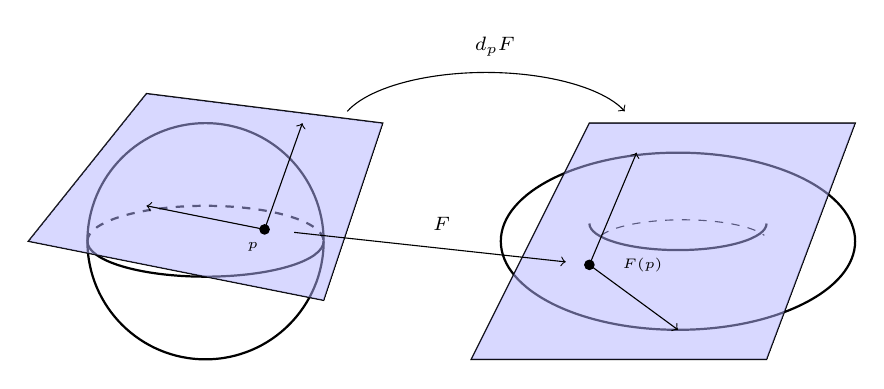
\begin{tikzpicture}[scale=1.5]
	% Esfera
	\draw [thick] (-1,0) arc (0:180:1 and -0.3);
	\draw [thick, dashed] (-3,0) arc (180:0:1 and 0.3);
	\draw [thick] (-2,0) circle (1);

	% Espacio Tangente a Esfera
	\draw [line width=0.5] (-3.5,0) -- (-2.5,1.25) -- (-0.5,1) -- (-1,-0.5) -- cycle;
	\draw [fill=blue!30!white,opacity=0.5, line width=0] (-3.5,0) -- (-2.5,1.25) -- (-0.5,1) -- (-1,-0.5) -- cycle;

	% Punto $a$
	\filldraw (-1.5,0.1) circle (0.04);
	\node at (-1.60,-0.05) {\tiny $p$};

	% Vector en $a$
	\draw [->] (-1.5,0.1) -- (-1.18,1);
	\draw [->] (-1.5,0.1) -- (-2.5,0.3);

	% Toro
	\draw [thick] (2,0) ellipse  (1.5 and 0.75);
	\draw [thick] (1.25,0.15) arc (0:-180:-0.75 and 0.225);
	\draw [dashed] (1.35,0.05) arc (20:160:-0.735 and 0.2);

	% Espacio tangente a Toro
	\draw [line width=0.5] (1.25,1) -- (3.5,1) -- (2.75,-1) -- (0.25,-1) -- cycle;
	\draw [fill=blue!30!white,opacity=0.5, line width=0] (1.25,1) -- (3.5,1) -- (2.75,-1) -- (0.25,-1) -- cycle;

	% Punto $F(a)$
	\filldraw (1.25,-0.2) circle (0.04);
	\node at (1.7,-0.2) {\tiny $F(p)$};

	% Vector en $F(a)$
	\draw[->] (1.25,-0.2) -- (1.65,0.75);
	\draw[->] (1.25,-0.2) -- (2,-0.75);

	% Lineas
	\draw[->] (-1.25,0.075) -- (1.05,-0.175);
	\node at (0,0.15) {\scriptsize $F$};


	\draw[->] (-0.8,1.1) arc (160:20:1.25 and 0.5);
	\node at (0.45,1.65) {\scriptsize $d_{p}F$};
\end{tikzpicture}

	\caption{Representación del diferencial de un mapa suave en un punto.}
\end{figure}
El diferencial $d_pF$ está bien definido dado que $F: M \to N$ y $f: N \to \R$ son funciones suaves, esto implica que $f \circ F: M \to \R$ será una función suave, por lo que $\omega(f \circ F)$ tiene sentido, la linealidad se tiene como consecuencia de que $\omega$ sea lineal y, por último, $d_pF(\omega): C^{\infty}(N) \to \R$ es una derivación en $F(p)$ dado que si $f, g \in C^{\infty}(N)$ entonces:

\begin{align*}
	d_pF(\omega)(fg) & = \omega((fg) \circ F)                                               \\
	                 & = \omega((f \circ F)(g \circ F))                                     \\
	                 & = (f \circ F)(p)\omega(g \circ F) + (g \circ F)(p) \omega(f \circ F) \\
	                 & = (f \circ F)(p)d_pF(\omega)(g) + (g \circ F)(p)d_pF(\omega)(f).
\end{align*}

A continuación, mostraremos algunas propiedades de los diferenciales de mapas suaves entre variedades, propiedades que son extensiones naturales de las propiedades conocidas de las derivadas totales del cálculo ordinario, como la linealidad del diferencial o la regla de la cadena.

\begin{lemma}\label{Lemma: Diferencial del Mapa Identidad}
	El diferencial del mapa identidad en una variedad es la identidad del espacio tangente a la variedad.
\end{lemma}

\begin{proof}
	Si $M$ es una variedad suave, $\id_M$ el mapa identidad en $M$, $p \in M$ un punto arbitrario y $\omega \in T_p(M)$ un vector tangente de $M$ en $p$, para cada $f \in C^{\infty}(M)$ se tiene:
	\begin{align*}
		d\id_{M}(\omega)(f) & = \omega(f \circ \id_M) = \omega(f).
	\end{align*}
	Dado que esto se cumple para cualquier $\omega \in T_p(M)$ y $f \in C^{\infty}(M)$, el diferencial será el mapa identidad en el espacio tangente.
\end{proof}

\begin{lemma}
	Si $M$ y $N$ son variedades suaves, $F: M \to N$ un mapa suave y $p \in M$ un punto arbitrario. El diferencial $d_pF: T_p(M) \to T_{F(p)}(M)$ es un operador lineal.
\end{lemma}

\begin{proof}
	Si $f,g \in C^{\infty}(N)$, $a \in \R$ y $\omega \in T_{p}(M)$, tenemos que:
	\begin{align*}
		d_pF(\omega)(af + g) & = \omega((af + g) \circ F)               \\
		                     & = \omega (af \circ F + g \circ F)        \\
		                     & = a\omega(f \circ F) + \omega(g \circ F) \\
		                     & = a d_pF (\omega)(f) + d_pF(\omega)(g).
	\end{align*}
	Por lo tanto, el diferencial de un mapa es un operador lineal.
\end{proof}

\begin{lemma}\label{Lemma: Regla de la Cadena para Diferenciales}
	Si $M$, $N$ y $P$ son variedades suaves, $F: M \to N$ y $G: N \to P$ mapas suaves y $p \in M$ un punto cualquiera, entonces el diferencial del mapa composición $G \circ F$ cumple la regla de la cadena, esto es,
	\[
		d_p(G \circ F) = d_{F(p)}G \circ d_pF
	\]
\end{lemma}

\begin{proof}
	Sea $\omega \in T_p(M)$ y $f \in C^{\infty}(P)$, tenemos que:
	\begin{align*}
		d_p(G \circ F) (\omega)(f) & = \omega(f \circ (G \circ F))       \\
		                           & = \omega ((f \circ G) \circ F)      \\
		                           & = d_pF(\omega)(f \circ G)           \\
		                           & = (d_{F(p)}G \circ d_pF)(\omega)(f)
	\end{align*}

	Por lo tanto, el diferencial de la composición cumple la regla de la cadena, más aún, es un mapa que lleva va del espacio tangente de $M$
	en $p$, $T_p(M)$, al espacio tangente de $P$ en $(G \circ F)(p)$, $T_{(G \circ F)(p)}(P)$.
\end{proof}

\begin{lemma}\label{Lemma: Diferencial de un Difeomorfismo}
	Si $M$ y $N$ son variedades suaves, $F: M \to N$ es un difeomorfismo y $p \in M$, entonces el diferencial $d_pF: T_p(M) \to T_{F(p)}(N)$ es un isomorfismo de espacios vectoriales y $(d_pF)^{-1} = d_{F(p)}(F^{-1})$.
\end{lemma}

\begin{proof}
	Dado que $F$ es un difeomorfismo, por definición $F$ es invertible por lo que existe una función $F^{-1}: N \to M$ tal que $F^{-1} \circ F = \id_M$ y $F \circ F^{-1} = \id_N$. Por los lemas probados anteriormente se tiene:
	\begin{align*}
		d_p(F^{-1} \circ F)      & = d_{F(p)}F^{-1} \circ d_pF = \id_{T_p(M)}       \\
		d_{F(p)}(F \circ F^{-1}) & = d_pF \circ d_{F(p)}F^{-1} = \id_{T_{F(p)}(N)}. \\
	\end{align*}
	Esto demuestra que tanto $d_pF$ como $d_{F(p)}F^{-1}$ son isomorfismos de espacios vectoriales dado que ambos son operadores lineales e invertibles, y además se comprueba que $(d_pF)^{-1} = d_{F(p)}F^{-1}$.
\end{proof}

De modo similar a la derivada total, el diferencial nos permitirá realizar cálculos en coordenadas locales, sin embargo, por cómo hemos definido al diferencial, estos operan sobre funciones definidas de manera global sobre la variedad. Al ser una generalización de la derivada total es de esperarse que puedan operar sin ambigüedad sobre subconjuntos abiertos, veremos esto a continuación.

\begin{lemma}
	Sea $M$ una variedad suave, $p \in M$ un punto arbitrario y $\omega \in T_{p}(M)$. Si $f,g \in C^{\infty}(M)$ coinciden en una vecindad de $p$, entonces $\omega(f) = \omega(g)$
\end{lemma}

\begin{proof}
	Definamos la función $h = f - g$, $h$ es una función suave que sea anula en una vecindad de $p$. Sea $\psi \in C^{\infty}(M)$ una función indicadora suave tal que $\psi(p) \equiv 1$ si $p \in \sup h$ y tal que $\sup \psi \subseteq M - \{p\}$. Dado que $\psi \equiv 1$ donde $h$ es diferente de cero, el producto $\psi h$ es idénticamente $h$. Y, como $h(p) = \psi(p) = 0$, por el lema \ref{Lemma: Propiedades De Las Derivaciones En Variedades} se tendrá que $\omega (h) = \omega (\psi h) = 0$.

	Por la linealidad de $\omega$ se sigue que $\omega(h) = \omega (f - g) = \omega(f) - \omega(g) = 0$, por lo tanto, $\omega(f) = \omega(g)$.
\end{proof}

\begin{lemma}\label{Lemma: Espacio Tangente a Subvariedad}
	Sea $M$ una variedad suave, $U \subseteq M$ un subconjunto abierto, y sea $\iota: U \to M$ el mapa de inclusión. Para cada $p \in U$, el diferencial $d_p\iota: T_p M \to T_pM$ es un isomorfismo de espacios vectoriales.
\end{lemma}

\begin{proof}
	Por el ejemplo \ref{Ex: Variedad Suave - Subvariedades Suaves} sabemos que $U$ es en sí misma una variedad suave por lo que no hay ambigüedad al considerar el espacio tangente en algún punto. La linealidad de la diferencial se tiene por definición de derivación.

	Para mostrar que el diferencial es inyectivo mostraremos que el kernel es nulo. Supongamos que $\omega \in T_{p}(U)$ y $d_p\iota(\omega) = 0 \in T_{p}(M)$. Sea $V$ una vecindad de $p$ tal que $\overline{V} \subset U$. Si $f: U \to \R$ es una función suave, por el lema \ref{Lemma: Lema de Extensión para Funciones Suaves} podemos garantizar que existe una función $\hat{f}: M \to \R$ que coincide con $f$ en $\overline{V}$. Luego, por el lema anterior se tiene que, como $f$ y $\hat{f}\big|_{U}$ son funciones suaves que coinciden en una vecindad de $p$, entonces:
	\begin{align*}
		\omega(f) & = \omega \left(\hat{f} \big|_{U} \right)\\
		          & = \omega(\hat{f} \circ \iota)   \\
		          & = d_p\iota(\omega)(\hat{f}) = 0
	\end{align*}

	Esto se cumplirá para cada función suave $f \in C^{\infty}(U)$, por lo que $\omega \equiv 0$, lo cual implica que $d\iota_p$ es inyectiva.

	Para mostrar que el diferencial del mapa de inclusión es sobreyectivo supongamos que $\omega \in T_p(M)$ es algún vector tangente arbitrario en $M$. Definamos al operador $\upsilon: C^{\infty}(U) \to \R$ de tal modo que $\upsilon(f) = \omega (\hat{f})$, donde $\hat{f}$ es cualquier función suave en $M$ que coincida con $f$ en $\overline{V}$, por el lema anterior $\upsilon(f)$ no depende de la elección de la función $\hat{f}$, por lo que $\upsilon$ está bien definida y es una derivación. Para cada función $g \in C^{\infty}(M)$ se cumple:
	\begin{align*}
		d_p\iota(\upsilon)(g)
		 & = \upsilon(g \circ \iota)                                  \\
		 & = \omega \left( (g \circ \iota) \big|_{V} \right) \\
		 & = \omega(g).
	\end{align*}
	Por lo tanto, $d\iota_p$ es un sobreyectivo, y por lo tanto será un isomorfismo entre los espacios vectoriales $T_p(U)$ y $T_p(M)$.
\end{proof}

\begin{theorem}[Invariancia de la Dimensión]\label{Teorema: Invariancia de la Dimensión}
	Si $M$ es una variedad suave, $n-$dimensional. Para cada $p \in M$, el espacio tangente $T_p(M)$ es un espacio vectorial $n-$dimensional.
\end{theorem}

\begin{proof}
	Para cada $p \in M$ podemos elegir una carta suave $(U, \phi)$ que contenga a $p$. Por definición $\phi$ es un difeomorfismo de $U$ a $\R^n$. El lema \ref{Lemma: Diferencial de un Difeomorfismo} nos dice que $T_{p}(U)$ y $T_{\phi(p)}(\R^n)$ son isomorfos, y el lema anterior garantiza que $T_{p}(U)$ y $T_{p}(M)$ también son isomorfos, por lo tanto, $T_{p}(M) \simeq T_{\phi(p)}(\R^n)$. De aquí que $\dim T_p(M) = \dim T_{\phi(p)}(\R^n) = n$.
\end{proof}

Una consecuencia inmediata del teorema \ref{Teorema: Isomorfismo entre Espacio Tangente y Espacio de Derivaciones} y el teorema anterior, es el siguiente corolario que nos da una identificación canónica de los elementos de cualquier espacio vectorial finito dimensional con los elementos de su espacio tangente, y, a su vez, dar una identificación canónica entre cada espacio tangente a un punto de una variedad y un espacio vectorial.

\begin{corollary}
	Sea $V$ un espacio vectorial finito dimensional con su estructura de variedad suave estándar. Para cada punto $a \in V$, el mapa $D_v: C^{\infty}(V) \to \R$ definido por:
	\[D_vf = \left. \frac{d}{dt} \right|_{t=0} f(a+tv), \]
	es un isomorfismo de $V$a $T_a(V)$.
\end{corollary}
